\documentclass[12pt]{article}
\usepackage[]{amsmath}
\usepackage[]{amsfonts}
\usepackage{amsthm}
\usepackage{graphicx}
\usepackage[]{geometry}
\newcommand*\oct{\vcenter{\hbox{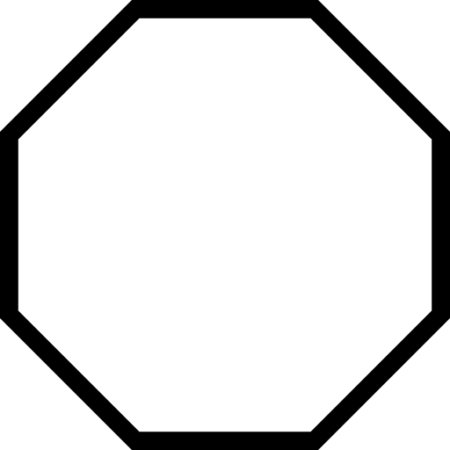
\includegraphics[width=.9em]{octagon.png}}}}
\usepackage[]{hyperref}

\newcommand{\F}{\mathcal{F}}
\newcommand{\Z}{\mathbb{Z}}

\newtheorem{theorem}{Theorem}
\newtheorem{lemma}{Lemma}
\newtheorem{proposition}{Proposition}
\newtheorem{conjecture}{Conjecture}
\newtheorem{corollary}{Corollary}

\theoremstyle{definition}
\newtheorem{definition}{Definition}

\title{Stopped Binary Strings}
\date{}

\author{Robert Dougherty-Bliss \\
    \href{mailto:robert.w.bliss@gmail.com}{robert.w.bliss@gmail.com} \\
    Charles Kenney \\
    \href{mailto:ctk47@math.rutgers.edu}{ctk47@math.rutgers.edu} \\
    Department of Mathematics, Rutgers University (New Brunswick) \\
    110 Frelinghuysen Rd. \\
    Piscataway, NJ 08854-8019, USA
}

\begin{document}
\maketitle

\begin{abstract}
    A binary string $(x_1, \dots, x_n)$ is \emph{stopped at index $k$} if all
    indices in $(k / 2, k]$ are zero. The \emph{stopping time} of a binary
    string is the smallest such $k$, if any exist. We show that the number of
    binary strings of length $2n$ with stopping time $2n$ is the $n$th
    Narayana--Zidek--Cappel number $T_n$. By considering binary expansions, we
    produce two new integer sequences (the ``stopped'' integers) and a
    measurable subset of the unit interval with unknown measure. Stating these
    results in arbitrary bases produces infinite families of integer sequences
    not in the OEIS, infinitely many new constants denoting the measures of
    certain subsets of the unit interval, and a generalization of the result
    that $T_n \sim c \cdot 2^n$.
\end{abstract}

\noindent A new, experimental machine is placed into a factory. The workers are
reluctant to trust this new contraption, which is surely intended to replace
them. They subject the machine to a rigorous \emph{testing} process: Once a
week, a worker will visit the machine and mark down a $1$ if any problem is
detected, and a $0$ otherwise. The first time the machine \emph{consecutively}
passes half of the total number of inspections, inspections will cease. This
process creates a \emph{binary string}, and the question is whether it ends in
sufficiently many $0$'s to denote a successful testing regimen. We call such
successful binary string \emph{stopped}.

Given a fixed number of inspections, how many binary strings are stopped? If we
inspect \emph{forever}, how many inspections will eventually result in a
stopped string? This paper explores some of these questions. Along the way we
will produce an infinite family of sequences which do not appear in the OEIS
and an infinite family of measurable sets on the real line whose measures are
unknown. First, let us give an explicit definition of stopped binary strings.

\begin{definition}
    A binary string $(x_1, x_2, \dots x_n)$ is \emph{stopped at index $k \leq
    n$} if $x_j = 0$ for all $j \in (k / 2, k]$. The \emph{stopping time} of a
    binary string is the smallest $k$ such that the string is stopped at index
    $k$, or $\infty$ if no such $k$ exists. Note that, except $1$ and $\infty$,
    every stopping time is even. We call a string of length $n$ with stopping
    time $n$ ``stopped'' without reference to an index.
\end{definition}

\begin{definition}
    Let $g(n)$ be the number of binary strings of length $n$ with stopping time
    $n$. 
\end{definition}

The motivating result for this paper is that the number of binary sequences of
length $2n$ with stopping time $2n$---that is, $g(2n)$---equals the $n$th
Narayana--Zidek--Cappel number $T_n$, defined by the recurrence
\begin{align}
    T_1 &= 1 \notag \\
    T_2 &= 1 \notag \\
    T_{2n} &= 2 T_{2n - 1} \tag{$n \geq 2$} \\
    T_{2n + 1} &= 2 T_{2n} - T_n. \tag{$n \geq 1$}
\end{align}
The sequence $T_n$ is A2083 in the OEIS \cite{oeis}, and was originally
introduced by Capell and Narayana \cite{capell1970knock,
narayana1969tournaments, narayana1979tournaments} as a means to enumerate
random knock-out tournaments.

Alongside this result, our definition of a stopped string generalizes to
various integer sequences and sets of reals by passing to the relevant binary
expansions. The definition also generalizes to bases other than $2$, the only
change being that any occurrence of ``$1$'' should be replaced with ``any
nonzero digit.'' This leads to an infinite family of sets, integer sequences,
and so on.

The authors have created a Maple package for studying stopped strings called
\texttt{stopTimes}. It is available as a git repository here:
\url{https://github.com/CTVKenney/stopTimes}.

The rest of this paper is organized as follows. Section~\ref{sec:recs}
establishes the identity between the number of stopped binary strings and the
Narayana--Zidek--Capell numbers, generalizes this result to arbitrary bases,
and gives some elementary results about the enumerating sequences.
Section~\ref{sec:reals} defines a set of reals in the unit interval whose
binary expansions are ``stopped,'' and considers the measure of this set.
Section~\ref{sec:integers} gives two new integer sequences and discusses their
natural densities.

\section{Counting stopped binary strings}
\label{sec:recs}

Since stopping times are even except for $1$, we know that $g(n)$ is zero
for all odd $n$ except $n = 1$, where $g(1) = 1$. Thus the interesting sequence
is $g(2n)$, which we will show (in two ways!) equals the
Narayana--Zidek--Capell sequence $T_n$.

It is convenient to work with \emph{infinite} binary strings which are nonzero
in only finitely many places. This is equivalent to studying finite binary
strings, but has the benefit that every such infinite string has a finite
stopping time when considered as a sufficiently long, finite binary string.

\begin{definition}
    Let
    \begin{equation*}
        V = \bigoplus_{k=1}^\infty (\Z/2\Z)
    \end{equation*}
    be the direct sum of infinitely many copies of $\Z / 2\Z$. That is, the set
    of all infinite tuples $(x_1, x_2, x_3, \dots)$ where each $x_k$ is $0$ or
    $1$, and only finitely many are $1$. For each positive integer $k$, let
    $\oct_k$ be the set of elements of $V$ which are zero beyond position $k$
    and, when the first $k$ entries are regarded as a finite binary string,
    they have stopping time $k$. (As a result, all entries after $k/2$ are 0.)
    That is, $\oct_1 = \{0\} \subset V$,
    \begin{equation*}
        \oct_{2k} = \{v \in V : \forall j > k, v_j = 0, \text{ and } v \text{ has stopping time } 2k \}
    \end{equation*}
    and $\oct_{2k + 1} = \emptyset$ for every integer $k \geq 1$.
\end{definition}

Note that $g(n) = |\oct_n|$ for every positive integer $n$.

\begin{theorem}
    The sequence $g(n)$ satisfies the recurrence
    \begin{align*}
        g(1) &= g(2) = g(4) = 1 \\
        g(4n) &= 2 g(4n - 2) \\
        g(4n + 2) &= 2 g(4n) - g(2n).
    \end{align*}
\end{theorem}

First, we will prove this directly from our definitions.

\begin{proof}
    Each nonzero element in $V$ has a final nonzero entry (equal to $1$). Let $e_0
    \colon V \to V$ be a map which inserts a $0$ in the position of this final
    entry, shifting the previous final entry to the right one space. Similarly,
    let $e_1$ insert a $1$. Symbolically,
    \begin{equation*}
        e_0(b) =
            \begin{cases}
                0 \text{ if } b=0 \\
                (b_1, ..., b_j, 0, 1, 0,0,...) \text{ if } b = (b_1, ..., b_j, 1, 0, 0, ...)
            \end{cases}
    \end{equation*}
    and
    \begin{equation*}
        e_1(b) =
            \begin{cases}
                (1, 0, 0, \dots) \text{ if } b=0 \\
                (b_1, ..., b_j, 1, 1, 0,0,...) \text{ if } b = (b_1, ..., b_j, 1, 0, 0, ...).
            \end{cases}
    \end{equation*}
    Note that $e_0$ and $e_1$ are injective, $e_0(V) \cap e_1(V) = \emptyset,$
    and $e_0(V) \cup e_1(V) = V.$

    For any positive integer $k$,
    \begin{equation*}
        \oct_{2k + 2} \subseteq e_0(\oct_{2k}) \cup e_1(\oct_{2k}).
    \end{equation*}
    Indeed, the final nonzero entry of every string in $\oct_{2k + 2}$ occurs
    at position $k + 1$. Removing the immediately preceding entry produces a
    string in $\oct_{2k}$---$e_0$ and $e_1$ simply add the entry back.

    In the other direction, for $k \geq 2$ we have
    \begin{equation*}
        e_1(\oct_{2k}) \subseteq \oct_{2k + 2},
    \end{equation*}
    because inserting a $1$ into position $k$ will never decrease the stopping
    time. For \emph{odd} $k \geq 3$ we have
    \begin{equation*}
        e_0(\oct_{2k}) \subseteq \oct_{2k + 2},
    \end{equation*}
    because inserting a $0$ at position $k$ will only decrease the stopping
    time if the new stopping time \emph{is} $k$; this is impossible if $k$ is
    odd. This shows that
    \begin{equation*}
        \oct_{2k + 2} = e_0(\oct_{2k}) \cup e_1(\oct_{2k}),
    \end{equation*}
    and thus
    \begin{equation*}
        g(2k + 2) = 2 g(2k)
    \end{equation*}
    for $k \geq 3$ odd.

    To handle the even case, let
    \begin{equation*}
        \oct_{2k}^1 = \{(b_1, ..., b_{2k}, 1, 0,0,...) \in V \text{ s.t. } (b_1,...,b_{2k},0,0,...) \in \oct_{2k}\}.
    \end{equation*}
    (Note that $|\oct_{2k}^1| = |\oct_{2k}| = g(2k)$.) Then
    \begin{equation*}
        e_0(\oct_{4k}) \subseteq \oct_{4k + 2} \cup \oct_{2k}^1.
    \end{equation*}
    This implies
    \begin{equation*}
        \oct_{4k + 2} \cup \oct_{2k}^1 = e_0(\oct_{4k}) \cup e_1(\oct_{4k}).
    \end{equation*}
    (That the left contains the right is clear given the preceding inclusion.
    For the other direction, note $\oct_{2k}^1 \subseteq
    e_0(\oct_{4k})$, since if $(b_1, ..., b_{2k}, 0,0,...) \in \oct_{2k}$ then
    $(b_1, ..., b_{2k-1},1,0,0,...)$ has stopping time precisely $4k$.) Therefore
    \begin{equation*}
        g(4k + 2) + |\oct_{2k}^1| = 2 g(4k),
    \end{equation*}
    or
    \begin{equation*}
        g(4k + 2) = 2 g(4k) - g(2k).
    \end{equation*}
    This establishes the recurrence.
\end{proof}

Now we will prove our theorem combinatorially by relating our sequence to a
certain class of compositions. Recall that a \emph{composition} of an integer
$n$ is a vector in $(\Z_{>0})^m$, for some $m \in \{1,2,...,n\}$, whose
components add to $n$. According to the OEIS, the $n$th Narayana-Zidek-Capell
number $T_n$ is the cardinality of the set
\begin{align*}
    R_n = \left\{ \text{Compositions } p \text{ of } n \text{ satisfying } p_1 = 1 \text{ and } p_k \leq \sum_{j=1}^{k-1} p_j \right\}.
\end{align*}

\begin{proposition}
    The number of stopped binary strings of length $2n$ are in bijection with
    the compositions in $R_n$.
\end{proposition}

\begin{proof}
    For $j \in \Z_{>0},$ let $f(j) = (0,0,...,0,1)$, with $j-1$ zeroes preceding the one.
    Then for $p \in (\Z_{>0})^m,$ let
    \begin{align*}
        F(p) = (f(p_1), f(p_2), ..., f(p_m), 0,0,...),
    \end{align*}
    concatenated in the natural way, with a tail of zeroes appended at the end.
    Then $F: R_n \overset{\sim}{\to} \oct_{2n}$ is a bijection, so $|\oct_{2n}| = g(2n) = T_n.$
    Indeed, if $p \in R_n$, then since $\sum_{j=1}^{m} p_j = n,$ the final nonzero entry in $F(p)$ is in spot $n$. Thus
    $F(p)$ is stopped at time $2n$, and is not stopped at time $t$ for any $t \in [n,2n-1].$
    And if the zeroes from $f(p_r)$ in $F(p)$ caused $F(p)$ to be stopped at some time $t \leq n-1,$
    \begin{align*}
        F(p) = (f(p_1), ..., f(p_{r-1}), 0,0,...,&0,...) \\
	&\uparrow \\
	&\text{index } t
    \end{align*}
    then $p_r  > \lceil t/2 \rceil \geq \sum_{j=1}^{r-1} p_j.$ But this would contradict the fact that $p \in R_n.$
    And, if $b \in \oct_{2n}$ has 1s at indices $a_1 = 1, a_2, ..., a_\ell = n,$ then
    \begin{align*}
	&F^{-1}: \oct_{2n} \to R_n \\
	&F^{-1} : b \mapsto (a_1, a_2 - a_1, a_3 - a_2, ..., a_\ell - a_{\ell-1})
    \end{align*}
    provides an inverse to $F$, since the index $a_r$ of the $r$th one in b is at most
    twice the index $a_{r-1}$ of the $(r-1)$st one.
\end{proof}

A slightly different recurrence holds for arbitrary bases. Let $g_b(n)$ be the
number of $b$-ary strings of length $n$ with stopping time $n$. Again, stopping
time $n$ means that all entries with indices in $(n/2, n]$ are 0, but for
$1\leq m<n,$ some entry in $(m/2, m]$ is nonzero. In the experimental machine
example, this corresponds to the case where there are $b-1$ distinct errors the
machine could throw. Then
\begin{align}
    g_b(1) &= 1 \notag \\
    g_b(2) &= b - 1 \notag \\
    g_b(4) &= (b - 1)^2 \notag \\
    g_b(4n) &= b g_b(4n - 2) \tag{$n \geq 2$}\\
    g_b(4n + 2) &= b g_b(4n) - (b - 1) g_b(2n) \tag{$n \geq 1$}.
\end{align}
The proof for arbitrary $b$ is nearly identical to $b = 2$.

It is cumbersome to always write $g_b(2n)$, so let us introduce an auxillary
sequence for convenience.

\begin{definition}
    Let $r_b(n) = g_b(2n)$ be the number of $b$-ary strings of length $2n$ with
    stopping time $2n$, for $n \geq 1$.
\end{definition}

The recurrences now read
\begin{align}
    r_b(1) &= b - 1 \notag \\
    r_b(2) &= (b - 1)^2 \notag \\
    r_b(2n) &= b r_b(2n - 1) \tag{$n \geq 2$} \\
    r_b(2n + 1) &= b r_b(2n) - (b - 1) r_b(n) \tag{$n \geq 1$}.
\end{align}

The sequences $r_b(n)$ seem new for $b \geq 3$ in the sense that they do not
appear in the OEIS. All $r_b(n)$ satisfy the following ``meta-Fibonacci''-like
property.

\begin{proposition}
    For all $b \geq 2$ and $n \geq 2$,
    \begin{equation*}
        r_b(n) = (b - 1) \sum_{k = 1}^{\lfloor n / 2 \rfloor} r_b(n - k).
    \end{equation*}
\end{proposition}

\begin{proof}
    The result holds for $n = 2$ since
    \begin{equation*}
        r_b(2) = (b - 1) \sum_{k = 1}^1 r_b(k).
    \end{equation*}
    For $2n \geq 4$, we can use induction to write
    \begin{align*}
        r_b(2n) &= (b - 1) r_b(2n - 1) + r_b(2n - 1) \\
                &= (b - 1) r_b(2n - 1) + (b - 1) \sum_{k = 1}^{n - 1} r_b(2n - 1 - k) \\
                &= (b - 1) \sum_{k = 1}^n r_b(2n - k).
    \end{align*}
    A similar argument applies for $2n + 1 \geq 3$.
\end{proof}

The recurrence of $r_b(n)$ implies that $r_b(n) = O(b^n)$, made sharper in the
following proposition.

\begin{proposition}
    \label{monotone}
    For every $b \geq 2$, $r_b(n) / b^n$ is monotonically decreasing. In
    particular,
    \begin{equation*}
        \frac{r_b(n)}{b^n} \leq \frac{b - 1}{b},
    \end{equation*}
    or
    \begin{equation*}
        \frac{g_b(2n)}{b^n} \leq \frac{b - 1}{b}
    \end{equation*}
    for $n \geq 1$.
\end{proposition}

\begin{proof}
    Since $r_b(n)$ is positive by definition, the recurrence for $r_b(n)$
    implies
    \begin{equation*}
        r_b(n) \leq b r_b(n - 1)
    \end{equation*}
    for all $n \geq 2$, which is equivalent to our claim that $r_b(n) / b^n$
    is monotonically decreasing. In particular,
    \begin{equation*}
        \frac{r_b(n)}{b^n} \leq \frac{r_b(1)}{b^1} = \frac{b - 1}{b},
    \end{equation*}
    as desired.
\end{proof}

This proposition implies that $r_b(n) / b^n$ converges to some nonnegative
constant. In the Narayana--Zidek--Capell case $b = 2$, the constant is
\emph{positive}. This was established by Narayana and Capell themselves
\cite{capell1970knock} and reproven by Emerson \cite{emerson2006family} using
the meta-Fibonacci property. In fact the constant is positive for all $b \geq
2$ as the following theorem indicates, so $r_b(n)$ grows at exactly the same
rate as $b^n$. 

\begin{theorem}
    There exist positive constants $c_b$ such that
    \begin{equation*}
        \lim_n \frac{r_b(n)}{b^n} = \lim_n \frac{g_b(2n)}{b^n} = c_b.
    \end{equation*}
    Further, for $b \geq 3$,
    \begin{equation*}
        c_b \geq \left(1 - \frac{1}{b}\right)^4.
    \end{equation*}
\end{theorem}

Here are approximations of these constants:
\begin{align*}
    c_2 &\approx 0.07917104341 \\
    c_3 &\approx 0.2525395027 \\
    c_4 &\approx 0.3889420714 \\
    c_5 &\approx 0.4874305959 \\
    c_6 &\approx 0.5599514923.
\end{align*}

\begin{proof}
    We will prove the slightly stronger claim that
    \begin{equation*}
        \frac{r_b(n)}{b^n} \geq c + \frac{C}{b^{n / 2}}
    \end{equation*}
    for $n \geq 4$, where
    \begin{equation*}
        C = \frac{b - 1}{b - \sqrt{b}} \frac{r_b(2)}{b^2}
        ; \quad
        c = \frac{r_b(4)}{b^4} - \frac{C}{b^2}.
    \end{equation*}
    The quantity $c$ is positive for $b \geq 2$, which amounts to the base case
    $n = 4$.

    For the inductive step, suppose that the claim holds for $n = 2k - 1 \geq
    4$. Then the recurrence for $r_b$ implies
    \begin{equation*}
        \frac{r_b(2k)}{b^{2k}} = \frac{r_b(2k - 1)}{b^{2k - 1}}
                               \geq c + \frac{C}{b^{k - 1 / 2}}
                               \geq c + \frac{C}{b^k},
    \end{equation*}
    which establishes the claim for $n = 2k$. If the claim holds for $n = 2k
    \geq 4$, then the recurrence for $r_b$ implies
    \begin{align*}
        \frac{r_b(2k + 1)}{b^{2k + 1}} &= \frac{r_b(2k)}{b^{2k}} - (b - 1) \frac{r_b(k)}{b^{2k + 1}} \\
                                       &\geq c + \frac{C}{b^k} - (b - 1)\frac{r_b(k)}{b^{2k + 1}}.
    \end{align*}
    To turn this lower bound into the desired one, it would suffice to check
    that
    \begin{equation*}
        \frac{C}{b^k} - (b - 1)\frac{r_b(k)}{b^{2k + 1}} \geq \frac{C}{b^{k + 1/2}},
    \end{equation*}
    or
    \begin{equation*}
        \frac{r_b(k)}{b^k} \leq \frac{b - \sqrt{b}}{b - 1} C.
    \end{equation*}
    Since $r_b(k) / b^k$ is monotonically decreasing and $k \geq 2$, we
    \emph{do} have
    \begin{equation*}
        \frac{r_b(k)}{b^k} \leq \frac{r_b(2)}{b^2} = \frac{b - \sqrt{b}}{b - 1} C,
    \end{equation*}
    which establishes the claim for $2k + 1$. Induction does the rest.

    To get the inequality, note that
    \begin{equation*}
        c = \left( 1 - \frac{1}{b} \right)^3 \left(1 - \frac{1}{b(b - \sqrt{b})}\right)
        \geq
        \left( 1 - \frac{1}{b} \right)^4
    \end{equation*}
    for $b \geq 3$.
\end{proof}

The uniform base case of $n = 4$ was found via experimentation with
the procedure \texttt{lowerBoundProof(b)} is our Maple package
\texttt{stopTimes}.

It would be nice to understand these constants better. For example, according
to the OEIS, $c_2$ is a multiple of the Atkinson--Negro--Santoro constant given
in Section 2.28 of Finch's book of mathematical constants
\cite{finch2003mathematical}. We have no other promising leads.

\section{Stopped reals in the unit interval}
\label{sec:reals}

Suppose we choose a binary string $(0.b_1 b_2 b_3 b_4 ...)_2$ uniformly at
random; that is, each bit $b_i$ has an equal probability of being 0 or 1,
independently of all the others.  What is the probability that the resulting
sequence has finite stopping time? There is a great chance it will be stopped
early, by picking $b_1=0, b_2=0,$ or $b_3 b_4 = 00.$ On the other hand, the
longer the string becomes without being stopped, the less likely any particular
bit being $0$ will make it stop. There are two salient differences between
considering stopping times for binary (and later $b$-ary) sequences and
stopping times in $\oplus_{i=1}^\infty (\Z/2\Z)$:
\begin{enumerate}
    \item Binary sequences most likely never terminate, i.e., there are likely
        an infinite number of $1$s.
    \item A real number in $[0,1]$ can have more than one binary expansion,
        one of which is stopped (by an infinite tail of 0s), the other of which
        may or may not be (with an infinite tail of 1s).
\end{enumerate}
Since the definition of ``stopped at time $k$'' depends only on the first $k$ bits in the expansion,
(1) won't cause trouble, and in fact leads to our probabilistic questions.
(2) is innocuous as well, at least for questions of probability: the set of \emph{dyadic} rationals
in $[0,1]$, i.e. those which have two distinct binary expansions, has measure 0.
However, to avoid confusion, all definitions that follow use the terminating binary expansion, when the two disagree.

\begin{definition}
    Let $S_k$ be the set of reals in $[0, 1]$ which have stopping time $k$ when
    regarded as an infinite binary string. Membership in this set is determined
    by examining only the first $k$ bits of a binary expansion, so $S_k$ is
    measureable (in fact, it is a union of half-open dyadic intervals). Let $S = \cup_{k \geq 1} S_k$ be the set of all stopped reals
    in $[0, 1]$, which is measurable since the $S_k$ are.
\end{definition}

Let us get a feel for what the sets $S_k$ ``look like.'' First, observe that
every element of $S_k$ consists of a binary string which has stopping time $k$
followed by \emph{any} binary string at all. Thus, each string with stopping
time $k$ determines an interval of length $2^{-k}$ included in $S_k$, and the
disjoint union of these intervals is \emph{all} of $S_k$. In this way, we can
compute the following sets:
\begin{align*}
    S_1 &= [0, 1/2) \\
    S_2 &= [1/2, 3/4) \\
    S_4 &= [3/4, 13/16) \\
    S_6 &= [7/8, 57/64) \\
    S_8 = [13/16, 209/256) &\cup [15/16, 241/256).
\end{align*}

\begin{figure}
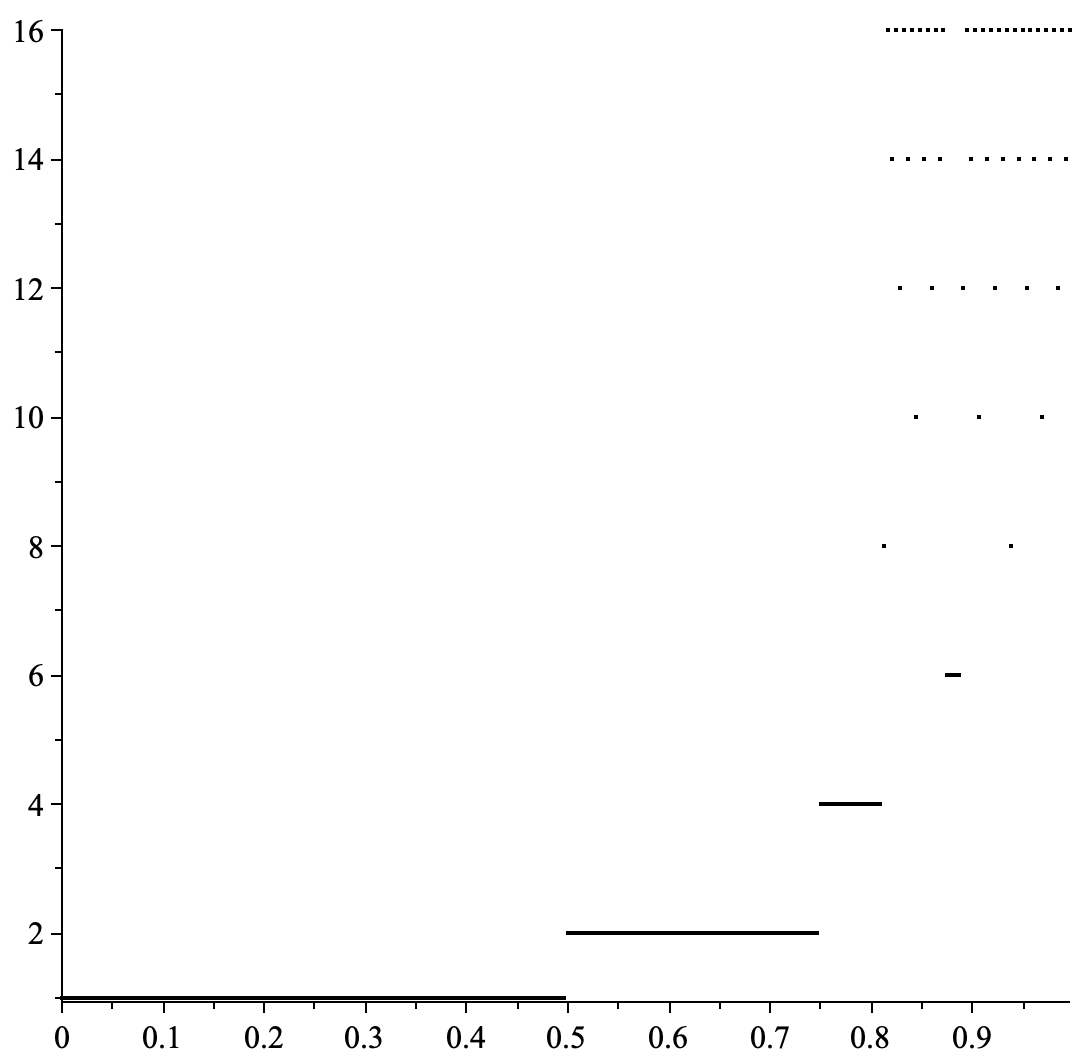
\includegraphics[width=\textwidth]{fig1.png}
\caption{Plot of binary sequence stopping times. Stopping times take values in $[0,\infty].$}
\end{figure}

This simple description of $S_k$ gives us a nice expression for the measure of
$S$.

\begin{theorem}
    Let $\beta_2$ be the measure of $S$. Then
    \begin{equation*}
        \beta_2 = \sum_{k \geq 1} \frac{g(k)}{2^k} = \frac{1}{2} + \sum_{k \geq 1} \frac{g(2k)}{4^k}
        \approx 0.841657913173647.
    \end{equation*}
\end{theorem}

\begin{proof}
    The measure of $S_k$ is $g(k) / 2^{2k}$, where $g(k)$ is the number of
    binary strings of length $k$ with stopping time $k$. Since $S$ is the
    pairwise disjoint union of the $S_k$, the ``exact'' result follows
    immediately.
\end{proof}

The constant $\beta_2$ seems new. We conjecture that it is irrational and even
transcendental, but we really know nothing about it. The only information we
have is that it is a value of the ordinary generating function of $g(n)$.

\begin{definition}
    Let
    \begin{equation*}
        G(z) = \sum_{k \geq 0} g(k) z^k = z + \sum_{k \geq 1} g(2k) z^{2k}
    \end{equation*}
    be the ordinary generating function of $g(n)$, and
    \begin{equation*}
        A(z) = \sum_{k \geq 1} T_k z^k
    \end{equation*}
    the ordinary generating function of $T_k$. Note that $G(z) = z + A(z^2)$.
\end{definition}

\begin{proposition}
    The generating function $A(z)$ is analytic on a disk of radius $1 / 2$
    centered at the origin and satisfies
    \begin{equation*}
        A(z) = \frac{z(1 - A(z^2))}{1 - 2z}.
    \end{equation*}
\end{proposition}

\begin{proof}
    The equation is a routine computation using the recurrence for the Narayana-Zidek-Capell numbers proved in
    the previous section. We have:
    \begin{align*}
        \sum_{k \geq 1} T_k z^k
            &= \sum_{k \geq 1} T_{2k} z^{2k} + \sum_{k \geq 0} T_{2k+1} z^{2k + 1} \\
            &= \sum_{k \geq 1} 2 T_{2k-1} z^{2k} + T_1 z + \sum_{k \geq 1} (2T_{2k} - T_k) z^{2k + 1} \\
            &= 2 z \sum_{k \geq 0} T_{2k+1} z^{2k + 1} + 2 z \sum_{k \geq 1} T_{2k} z^{2k} - z A(z^2) + z \\
            &= 2z A(z) + z(1 - A(z^2)).
    \end{align*}
    Solving this for $A(z)$ yields the result. Since $T_n =
    O(2^n)$, we see that $A(z)$ converges everywhere that $\sum_{k \geq 0} (2z)^k = (1 -
    2z)^{-1}$ does, which is at least a disk of radius $1/2$.
\end{proof}

It is clear that
\begin{equation*}
    \beta_2 = G(1/2) =\frac{1}{2} + A(1/4).
\end{equation*}
But again, this is very little information. We suspect that neither $A(z)$ nor
$G(z)$ are algebraic.

Expanding reals in $[0, 1]$ with different bases yields different ``stopped
sets'' and different measures. The same arguments apply, except now the measure
of the $S_{b,k}$ will be $g_b(k) / b^k$. Thus, the measure of the set of $b$-ary
stopped reals is
\begin{equation*}
    \beta_b = \frac{1}{b} + \sum_{k \geq 1} \frac{g_b(2k)}{b^{2k}}.
\end{equation*}
These constants go as follows:
\begin{align*}
    \beta_2 &\approx 0.84165791317364708989 \\
    \beta_3 &\approx 0.62119074589923243760 \\
    \beta_4 &\approx 0.48141057151328202149 \\
    \beta_5 &\approx 0.39071175514852239829 \\
    \beta_6 &\approx 0.32805820924751380527.
\end{align*}
These seem to be decreasing, and indeed they are, down to 0.
(As the number of possible errors for the experimental machine increases, the probability
that it will run $n/2$ consecutive errorless weeks tends to 0.)

\begin{theorem}
    For $b \geq 2$,
    \begin{equation*}
        \frac{2}{b} - \frac{1}{b^2} \leq \beta_b \leq \frac{2}{b}.
    \end{equation*}
\end{theorem}

\begin{proof}
    The definition of $g_b$ shows that it is positive, and the recurrence
    established in the previous section shows that $g_b(2k) / b^k$ is
    monotonically decreasing. In particular,
    \begin{equation*}
        g_b(2k) / b^k \leq g_b(2) / b = \frac{b - 1}{b}.
    \end{equation*}
    for $k \geq 1$. Therefore
    \begin{equation*}
        \beta_b \leq \frac{1}{b} + \frac{b - 1}{b} \sum_{k \geq 1} \frac{1}{b^k}
        = \frac{2}{b}.
    \end{equation*}
    The lower bound is from the definition of $\beta_b$.
\end{proof}

\section{Stopped integers}
\label{sec:integers}

In this section we define two integer sequences related to stopped binary
strings. They are the \emph{maximally stopped} and \emph{prestopped} integers.

\begin{definition}
    A positive integer $n$ is \emph{maximally stopped} provided that its binary
    expansion has stopping time equal to its length. A positive integer $n$ is
    \emph{prestopped} if its binary expansion has length $k$ and is the prefix
    of a binary string with stopping time $2k$.
\end{definition}

The maximally stopped integers begin
\begin{equation*}
    2, 12, 56, 208, 240, 864, 928, 992, 3392, 3520, 3648, \dots,
\end{equation*}
and the prestopped integers begin
\begin{equation*}
    2, 4, 5, 8, 9, 10, 11, 12, 16, 17, 18, 19, 20, 21, 22, 23, 24, 25, 32, 33, \dots
\end{equation*}
Neither sequence appears in the OEIS.

\begin{definition}
    Let $M(x)$ and $P(x)$ be the number of maximally stopped and prestopped
    integers $\leq x$, respectively.
\end{definition}

\begin{proposition}
    \begin{equation*}
        P(x) = M(x^2)
    \end{equation*}
\end{proposition}

\begin{proof}
    There is a bijection between the prestopped integers $\leq x$ and the
    maximally stopped integers $\leq x^2$: Given a prestopped integer of binary
    length $k$, append $k$ zeros. Its inverse: Given a maximally stopped
    integer of binary length $2k$, remove $k$ zeros. To see that this is a
    bijection between the right intervals, choose a prestopped integer $n \geq
    x$ of binary length $k$. That is, $2^k \leq n < 2^{k + 1}$. Appending $k$
    zeros is done by multiplying by $2^k$, and $2^k n \leq x \cdot x = x^2$.
    The other direction is similar.
\end{proof}

\begin{proposition}
    The counting functions $M(x)$ and $P(x)$ satisfy
    \begin{align*}
        M(x) &= \Theta(\sqrt{x}) \\
        P(x) &= \Theta(x).
    \end{align*}
\end{proposition}

\begin{proof}
    Since $M(x) = M(\lfloor x \rfloor)$, suppose that $x$ is an integer and
    write $x = 2^m + k$ for an integer $m \geq 0$ and $0 \leq k < 2^m$. Every
    maximally stopped integer not exceeding $x$ has a binary expansion with
    length not exceeding $m + 1$. Conversely, every such binary string
    corresponds to a unique maximally stopped integer. Every such string with
    length less than $m + 1$ corresponds to an integer $< x$, so
    \begin{equation*}
        M(x) \geq \sum_{k < m + 1} g_2(k).
    \end{equation*}
    On the other hand, every integer counted by $M(x)$ has length $\leq m + 1$,
    so
    \begin{equation*}
        M(x) \leq \sum_{k \leq m + 1} g_2(k).
    \end{equation*}
    Since $g_2(2k) = \Theta(2^k)$, the upper bound and lower bounds are both
    $\Theta(2^{m / 2}) = \Theta(\sqrt{x})$. For example, there exists a
    positive constant $c$ such that $g_2(2k) \leq c 2^k$, so
    \begin{align*}
        \sum_{k \leq m + 1} g_2(k) &= \sum_{2k \leq m + 1} g_2(2k) \\
                                   &\leq \sum_{k \leq (m + 1) / 2} c 2^k \\
                                   &= O(2^{m / 2}) \\
                                   &= O(\sqrt{x}).
    \end{align*}
    The lower bound is treated similarly. It follows that $M(x) =
    \Theta(\sqrt{x})$, and therefore $P(x) = M(x^2) = \Theta(x)$.
\end{proof}

An easy corollary of this result is that the maximally stopped integers grow
like squares. That is, the $n$th maximally stopped integer is $\Theta(n^2)$. To
establish, say, the lower bound, let $m$ be the $n$th maximally stopped
integer, and note that
\begin{equation*}
    n = M(m) \leq c \sqrt{m}
\end{equation*}
for some constant $c$. Then $m \geq n^2 / c^2$. The upper bound is the same
except for the constant.

\begin{corollary}
    The maximally stopped integers have natural density $0$, i.e.,
    \begin{equation*}
        \lim_{x \to \infty} \frac{M(x)}{x} = 0.
    \end{equation*}
\end{corollary}

\begin{proof}
    Since $M(x) = \Theta(\sqrt{x})$, we have $M(x) / x = \Theta(x^{-1/2})$.
\end{proof}

\section{Conclusions and open questions}
\label{sec:conclusion}

We have produced infinite families of integer sequences, $r_b(n)$ and $g_b(n)$,
two infinite families of real constants, $c_b$ and $\beta_b$, and two new
integer sequences, the maximally stopped and prestopped integers.

It would be interesting to know more about the constants $c_b$ and $\beta_b$.
We can approximate them with the underlying recurrences and series
representations, but that is about all we can say. Are they expressible in
terms of well-known constants such as $e$, $\pi$, and $\gamma$? Are they
irrational? Transcendental? Has anyone ever seen them before? It seems unlikely
that they are well-known, or that we could say anything non-trivial about them
without significant amounts of sweat.

\begin{thebibliography}{1}

\bibitem{capell1970knock}
P.~Capell and T.~V.~Narayana, On knock-out tournaments. \emph{Canadian
Mathematical Bulletin} \textbf{13} (1970), 105--109.

\bibitem{emerson2006family}
N.~Emerson, A family of meta-Fibonacci sequences defined by variable order
recursions, arXiv preprint math/0508522 (2005).

\bibitem{finch2003mathematical}
S.~Finch, \emph{Mathematical Constants}, Cambridge university press, 2003.

\bibitem{narayana1969tournaments}
T.~V.~Narayana and J.~Zidek, Contributions to the Theory of Tournaments Part I
The Combinatorics of Knock-Out Tournaments. \emph{Cahiers du Bureau
universitaire de recherche op\'erationnelle S\'erie Recherche} \textbf{13}
(1969) 3--18.

\bibitem{narayana1979tournaments}
T.~V.~Narayana and F.~Agyepong, Contributions to the Theory of Tournaments Part
IV A Comparaison of Tournaments Through Probabilistic Completions.
\emph{Cahiers du Bureau universitaire de recherche op\'erationnelle S\'erie
Recherche} \textbf{32} (1979), 21--34.

\bibitem{oeis}
OEIS Foundation Inc., The On-Line Encyclopedia of Integer Sequences,
\url{http://oeis.org} (2021).

\end{thebibliography}

\end{document}
